\documentclass[10pt]{beamer}

\usetheme{metropolis}

\usepackage{appendixnumberbeamer}
% \includeonlyframes{applications}
\usepackage{multicol}
\usepackage{color}
\usepackage{emoji}

\usepackage{amsmath}
\usepackage{subcaption}
\DeclareMathOperator*{\argmax}{arg\,max}
% dope docs http://mirrors.ibiblio.org/CTAN/macros/latex/contrib/beamer-contrib/themes/metropolis/doc/metropolistheme.pdf#page8
\usepackage[style=phys,citestyle=numeric,backend=bibtex]{biblatex}
% https://tex.stackexchange.com/questions/167665/multiple-references-with-footfullcite to hv multiple footnoterefs
% \renewcommand\multicitedelim{\addsemicolon\space}
\renewcommand{\footnotesize}{\tiny} % change fontsize for footnotes
\addbibresource{../paper/refs.bib}

\definecolor{osuorange}{rgb}{0.84,0.25,0.035}
\setbeamercolor{frametitle}{bg=white, fg=normal text.fg}
\setbeamercolor{title separator}{fg=osuorange, bg=white}
\usepackage{booktabs}


\usepackage[font=scriptsize]{caption}
\captionsetup{labelformat=empty, justification=centering,font=scriptsize,labelfont=scriptsize}% redefines the caption setup of the figures environment in the beamer class.
\setbeamerfont{caption}{size=\tiny}        
% \addtobeamertemplate{frametitle}{}{\vspace{-\baselineskip}}
    
% change background color
\setbeamercolor{background canvas}{bg=white}
\newcommand{\data}{$(s_1, ..., s_k)$\xspace}

\usepackage{xspace}
\newcommand{\themename}{\textbf{\textsc{metropolis}}\xspace}

\title{the German tank problem}
\subtitle{a Bayesian treatment}
% \date{\today}
\author{Cory M. Simon}
\institute{
	Assistant Professor\\
	School of Chemical, Biological, and Environmental Engineering\\
	Oregon State University\\
	\texttt{simonensemble.github.io} \\
	\texttt{@CoryMSimon}
}
\date{}
\titlegraphic{\hfill
\includegraphics[height=1.0cm]{logo.png}}

\begin{document}
\maketitle

\section{historical context}

\begin{frame}[t]{World War II (1939-1945)}
	\begin{figure}
		\centering
		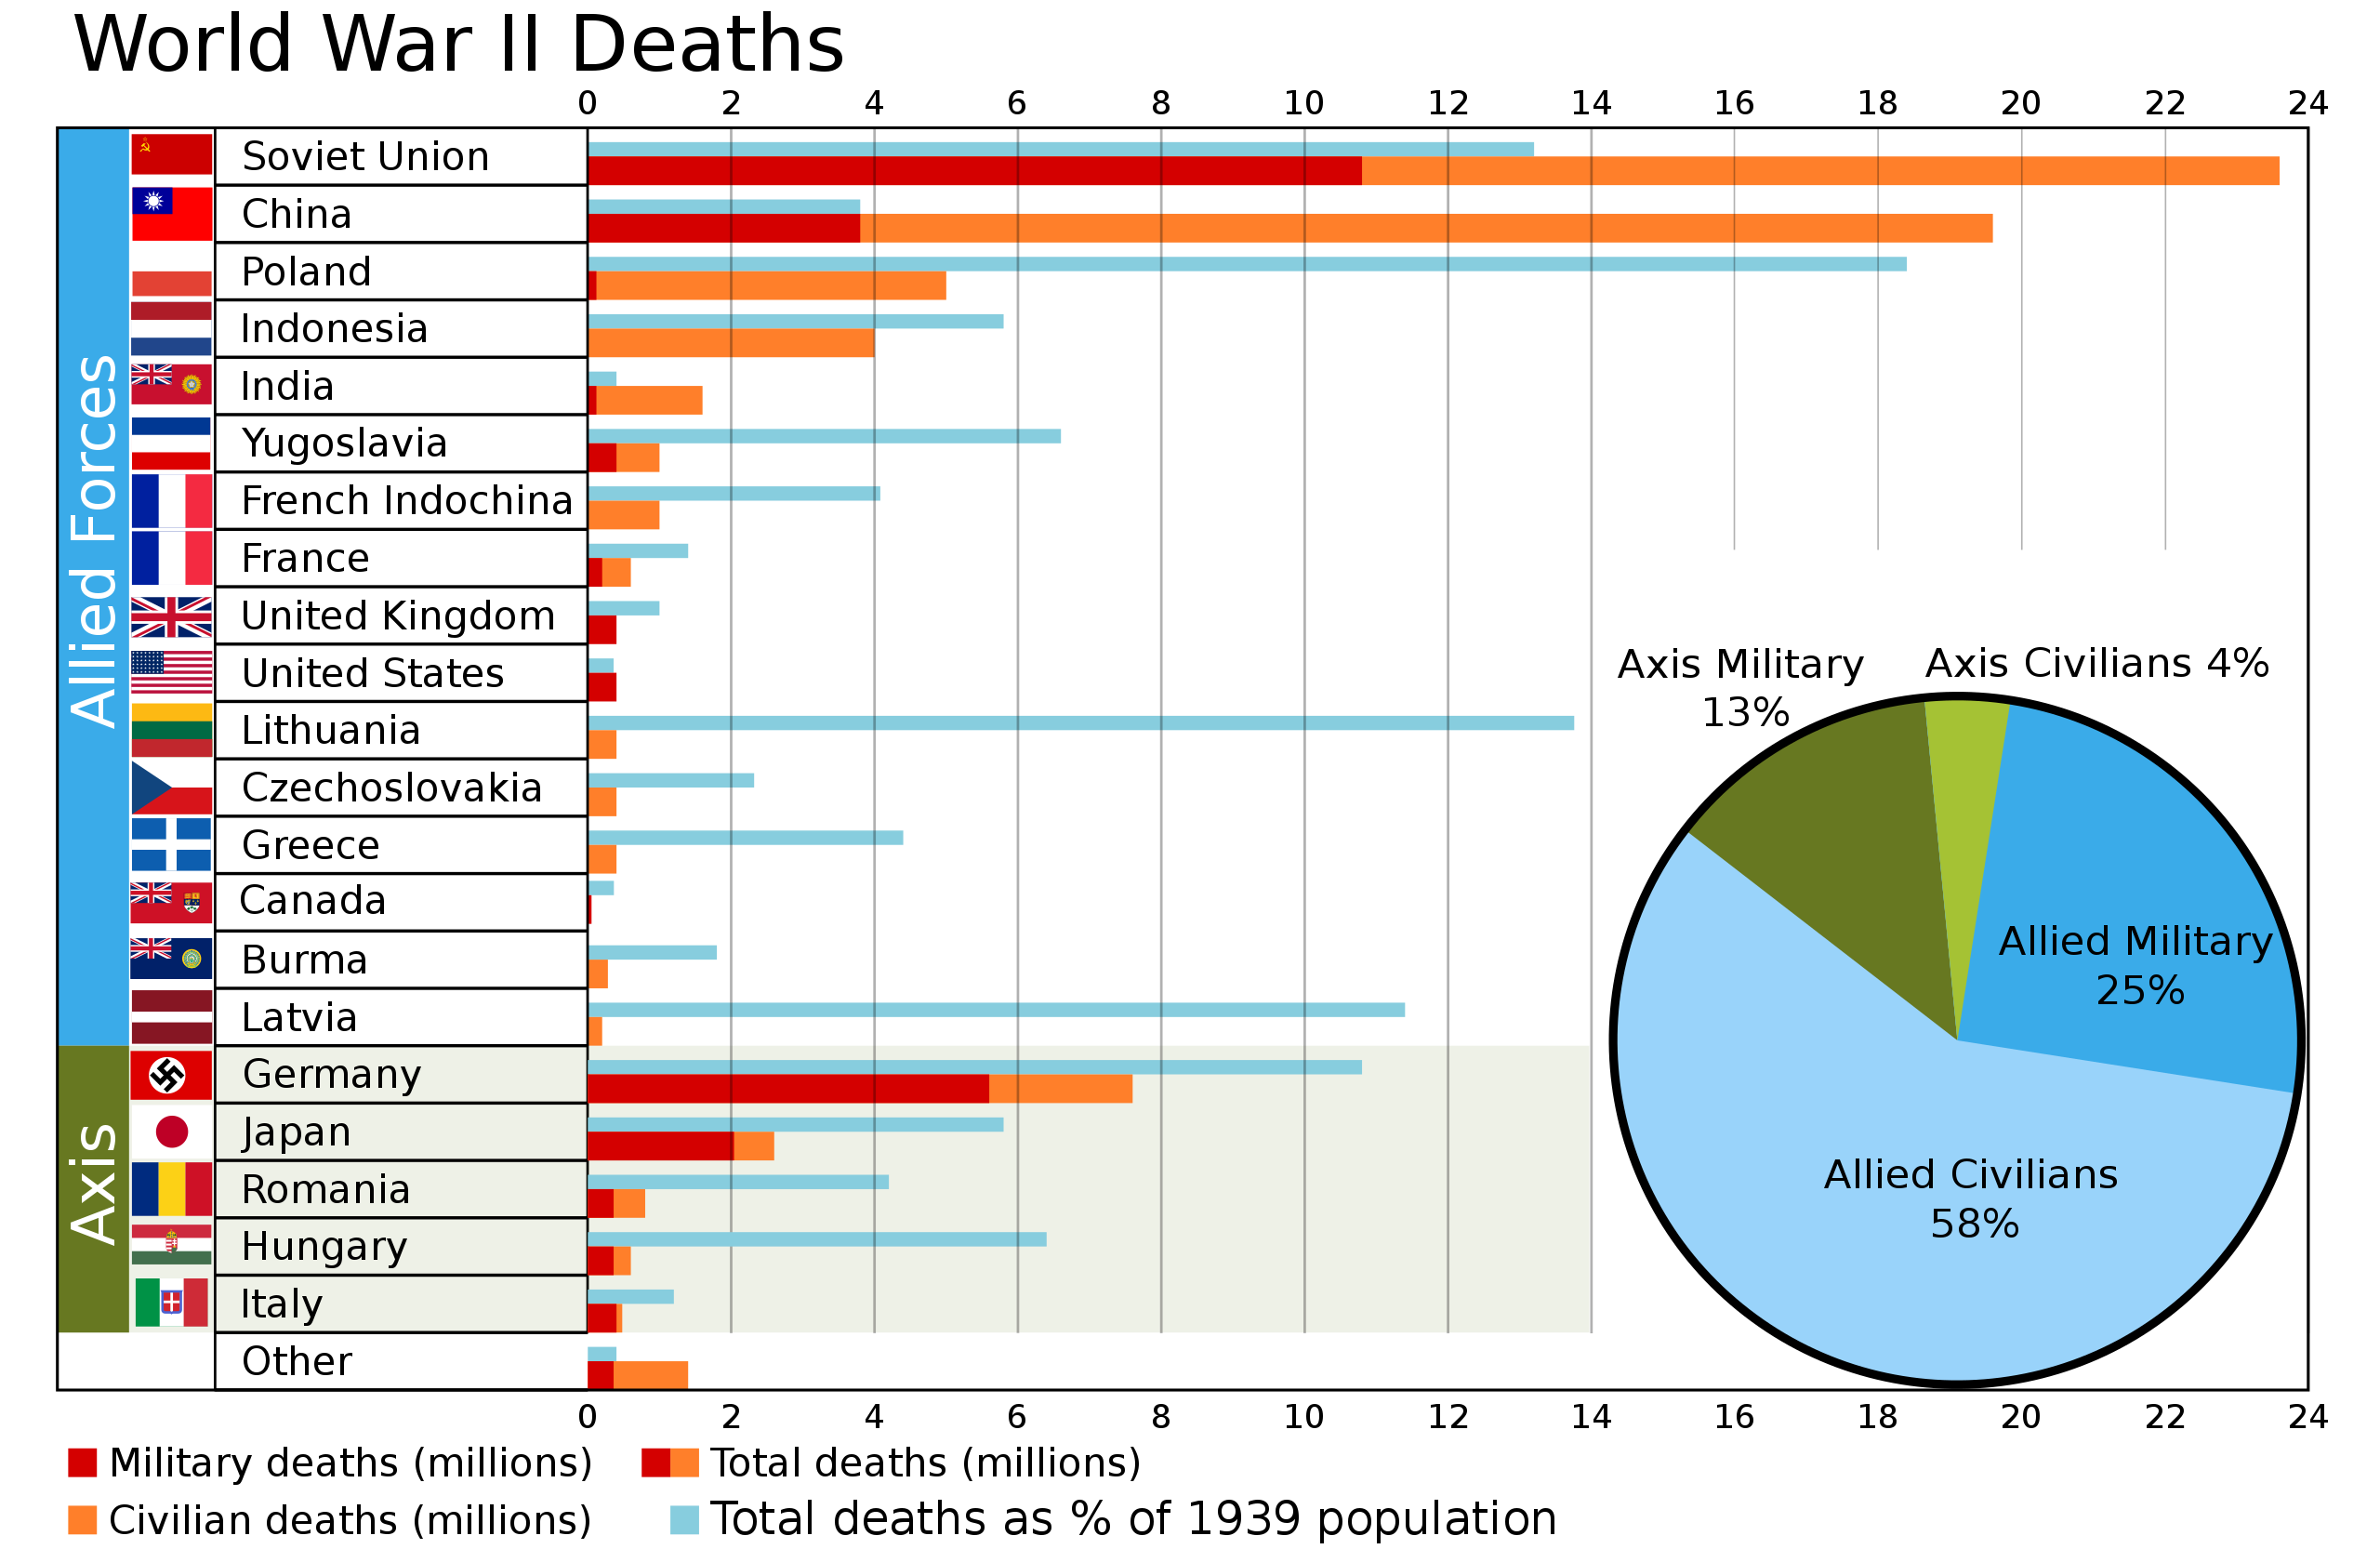
\includegraphics[width=0.85\textwidth]{WWII_deaths.png}
		\caption{source: Wikipedia}
	\end{figure}
\end{frame}

\begin{frame}[t]{estimating Germany's armament production}
	\alert{context:} the Allies wish to estimate Germany's production of tanks, tires, rockets, etc. 
	
	\begin{figure}
		\centering
		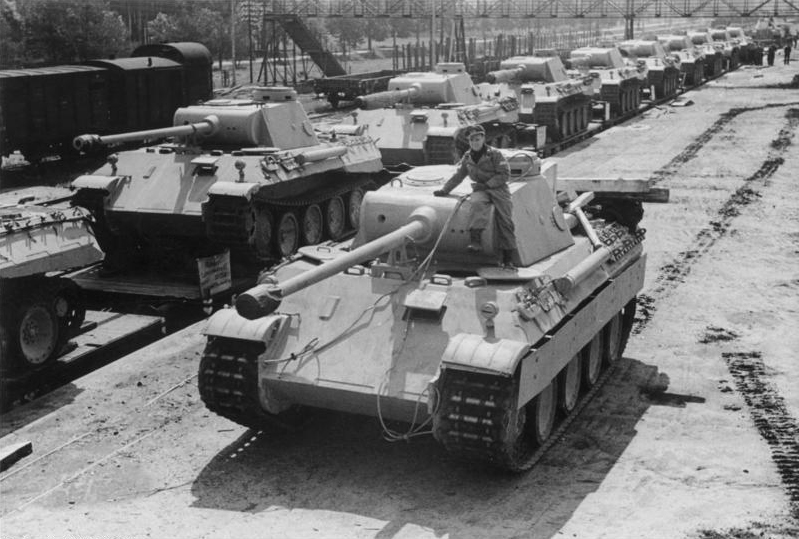
\includegraphics[width=0.4\textwidth]{panther_tank.jpg}
		\caption{the German Panther tank. source: Wikipedia}
	\end{figure}

	\pause
	
	conventional methods were unreliable and/or contradictory.
	\begin{itemize}
		\item extrapolating prewar manufacturing capabilities
		\item reports from secret sources
		\item interrogating prisoners of war
	\end{itemize}
\end{frame}

\begin{frame}[t]{Germany's practice of inscribing military equipment with serial numbers}
	Germany marked their military equipment with serial numbers and codes for the date and/or place of manufacture to:
	\begin{itemize}
		\item facilitate handling spare parts
		\item trace defective equipment/parts back to the manufacturer for quality control.
	\end{itemize}
	
	\pause 
	
	\emoji{bulb}  in 1943, these markings on a captured sample of German equipment conveyed information to British and American economic intelligence agencies about Germany's production of it.
\end{frame}

\begin{frame}[t]{serial number analysis for German tank production}
	
	\begin{table}[h!]
	\small
		\centering 
		\caption{Monthly production of tanks by Germany.} 	
\begin{tabular}{p{1.6cm} p{2.5cm} p{2.5cm} p{2cm}}
\toprule
 & \multicolumn{2}{c}{estimates} &   \\ 
\cmidrule(r){2-3}
date & conventional intelligence &  \only<2-3>{serial number analysis}  & \only<3>{German records} \\
\midrule
Jun. 1940 & 1000&  \only<2-3>{169} &  \only<3>{122} \\
Jun. 1941 &1550 &  \only<2-3>{244} &   \only<3>{271} \\
Aug. 1942 & 1550&  \only<2-3>{327}  & \only<3>{342} \\
\bottomrule
\end{tabular}
\end{table}

see Ruggles and Brodie \footfullcite{ruggles1947empirical} for the detailed historical account.

\end{frame}

\section{the German tank problem}

\begin{frame}[t]{the German tank problem}
\begin{alertblock}{problem statement}
the German military has $n$ tanks. 
each tank is inscribed with a unique serial number in $\{1, ..., n\}$. \newline

as the Allies, we do not know $n$, but we captured (without replacement) a sample of $k$ tanks with serial numbers \data. 

\begin{center}
	\begin{tabular}{cccc}
		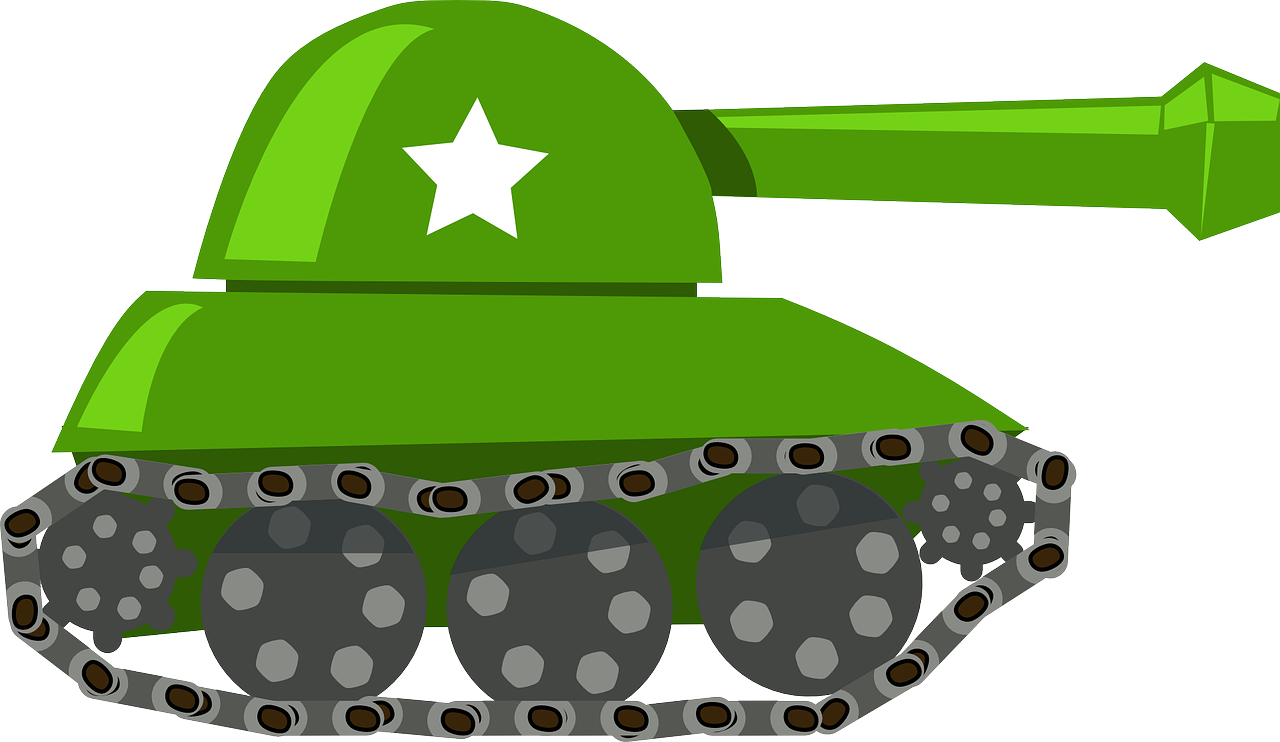
\includegraphics[width=0.125\textwidth]{../paper/tank.png} &  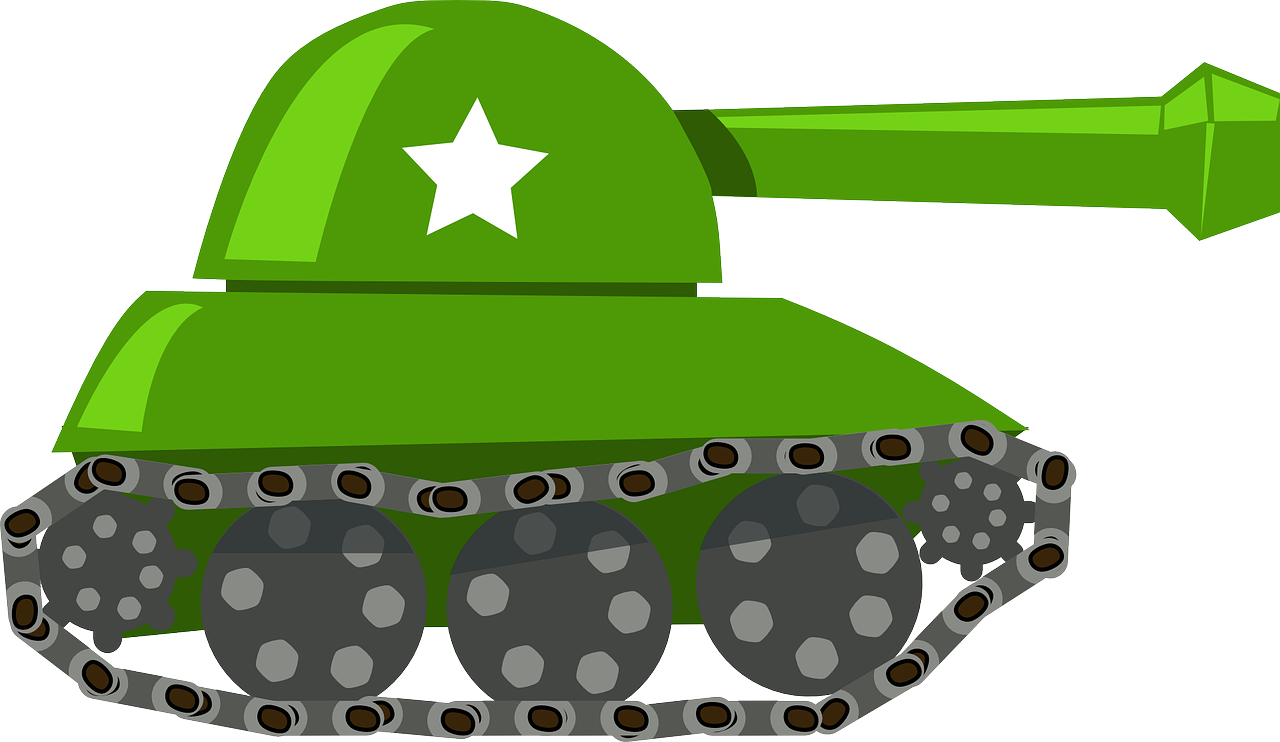
\includegraphics[width=0.125\textwidth]{../paper/tank.png}  & & 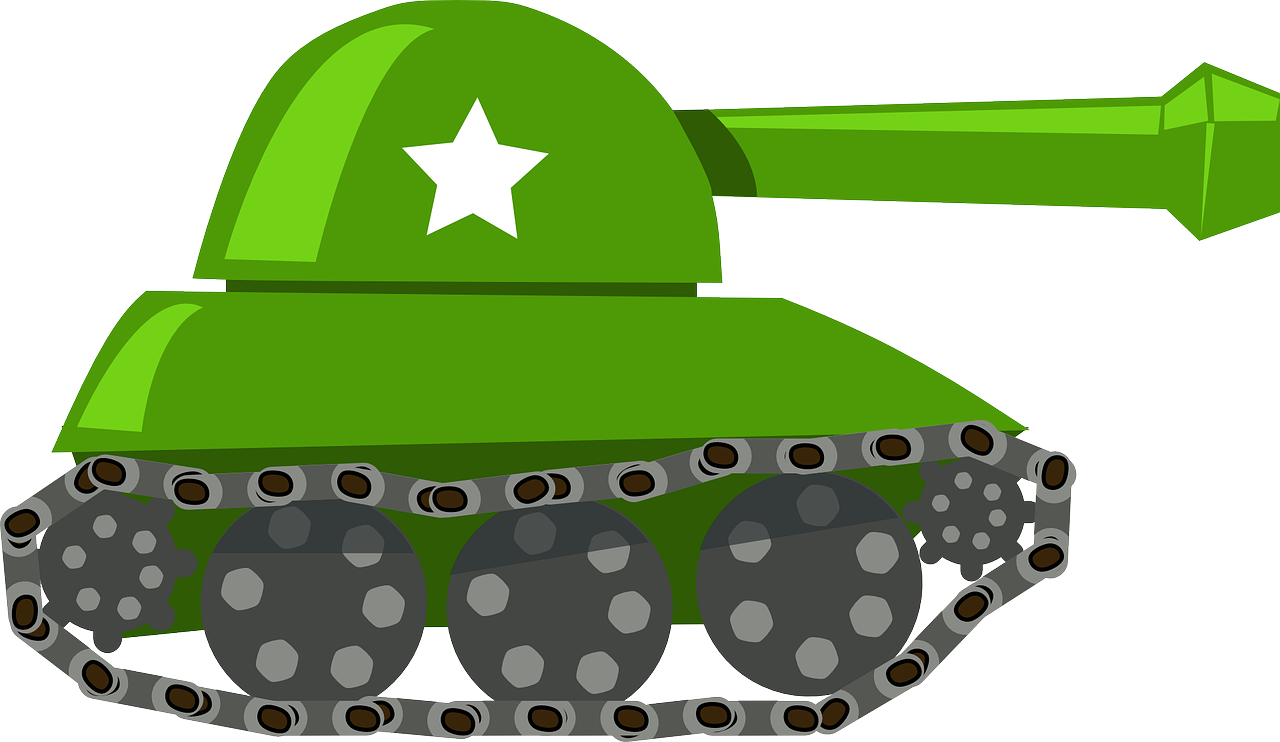
\includegraphics[width=0.125\textwidth]{../paper/tank.png} \\
		\large $s_1$ & \large $s_2$ & \large $\cdots$ & \large $s_k$ 
	\end{tabular}
\end{center}


\alert{objective}: estimate $n$ in consideration of the data \data.

\end{alertblock}
\pause 

\alert{key assumption}: all tanks in the population were equally likely to be captured.
\end{frame}

\begin{frame}[t]{the German tank problem}

\begin{figure}
	\centering
	\begin{subfigure}[b]{0.45\textwidth}
		\centering
		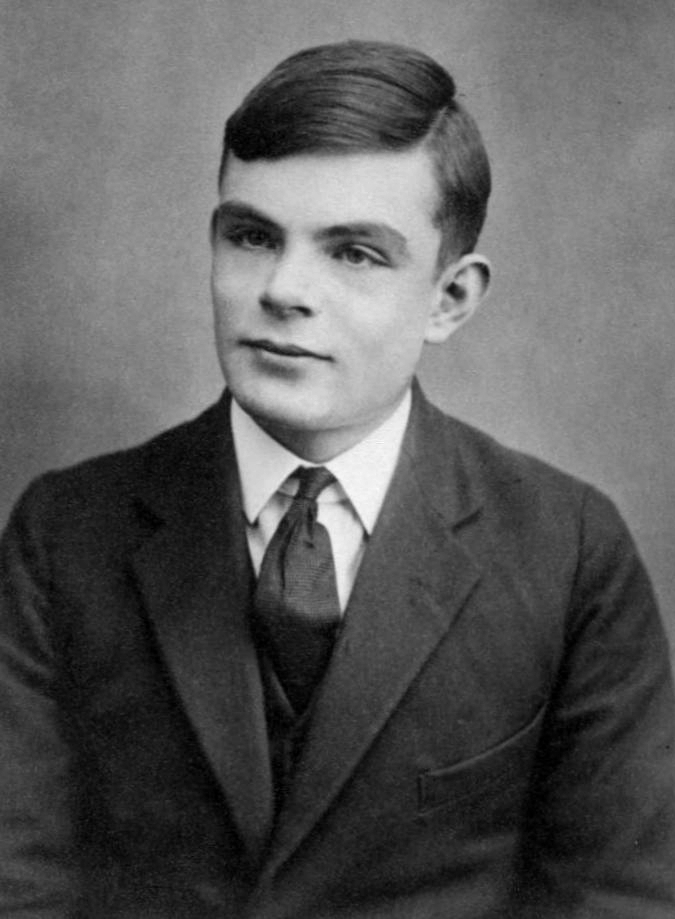
\includegraphics[height=0.5\textwidth]{turing.jpg} \caption{Alan Turing}
	\end{subfigure} 
	\begin{subfigure}[b]{0.45\textwidth}
		\centering
		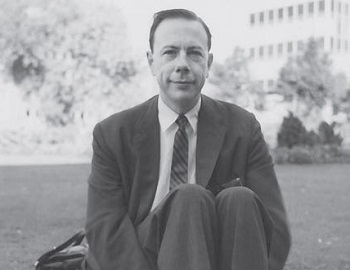
\includegraphics[height=0.5\textwidth]{gleason.jpg}  \caption{Andrew Gleason}
	\end{subfigure} 
\end{figure}


\begin{exampleblock}{origins?}
In 1942, Alan Turing and Andrew Gleason discussed a variant of the German tank problem, ``how to best to estimate the total number of taxicabs in a town, having seen a random selection of their license numbers'', in a crowded restaurant in Washington DC \footfullcite{hodges2014alan}$^,$\footfullcite{hall2014alan}. 
\end{exampleblock}
\end{frame}

\begin{frame}[t]{example}
\begin{figure}
	\centering
	\includegraphics[width=0.7\textwidth]{../paper/the_sample.pdf}
	\caption{the data $(s_1, s_2, s_3)$.}
\end{figure}

what is your estimate of $n$?
\end{frame}

\begin{frame}[t]{quantifying uncertainty in the tank population size}
any estimate of the tank population size $n$ from the data \data is subject to uncertainty.

\emoji{thinking} \emoji{question}
  
quantifying uncertainty in our estimate of $n$ is important because high-stakes military decisions may be made on its basis.
\end{frame}
\end{document}
